\documentclass[a4paper,11pt]{jreport}
\usepackage{masterthesis}
\usepackage[dvipdfmx]{graphicx}
\usepackage{url}
\graphicspath{ {./figure/} }

%次の行を有効にすると、その章だけが読み込まれる
%\includeonly{introduction}

%----------------------------------------------------------------------
% タイトルページ
%----------------------------------------------------------------------
% タイトル 2行にわたる場合は適宜改行をいれること。
\title{拡張現実感を用いた看板画像からの\\店舗情報アクセス手法に関する研究}

% 提出年月
\date{平成 31 年 2 月}

% 執筆者
\author{北村 茂生}
%----------------------------------------------------------------------

%\includeonly{introduction,design_guidline}

\begin{document}

%タイトルページ
\maketitle

\pagenumbering{roman}
\include{abstract}

%目次
\tableofcontents

%----------------------------------------------------------------------
%本文
%----------------------------------------------------------------------
\newpage
\pagenumbering{arabic}

\chapter{序論}
\label{chapter:introduction}

本章では,本研究の実施に至った背景を説明し,対象とする課題を明確にする.

%------------------------------------------------------------------------
\section{本研究の背景}
  \subsection{街中における看板}
  \label{subsection:signboards_in_town}
    現在,都市には多種多様な視覚情報が溢れている.
    都市に多く存在する視覚情報の1つとして,屋外広告物である看板が挙げられる.
    看板の目的は,看板を掲示する場所に存在する店舗や会社の名称の掲示が主である.
    店舗は不特定多数の人々に対して来店を訴求するために看板を掲示し,人々は目に入った看板に描かれているデザインや文字から何らかの影響を受けて,具体的な行動に移す\cite{Koyama:2016}.
    例えば,人々が都市空間において店舗を探す際,看板に描かれている内容から,飲食店や衣料販売店などの店舗の種類を判別し,どの店に入るかなどの意思決定を行っている.
    しかし,繁華街など店舗が多数存在する地域においては,都市環境への配慮が十分でなく,「目立つこと」「インパクトがあること」「興味を引くこと」が優先され,看板やネオンによって埋め尽くされた景観が形成されている場合がある\cite{Yokokawa:2000}.
    このような場合においては,看板がひしめき合うことで,逆に視覚情報が見えにくくなるという現象を引き起こしている\cite{Watanabe:2003}.
    そのため,看板が街を行き交う歩行者に対して情報を与えるという本来の役割を果たせていないという問題がある.

    また,看板から得られる情報は限定的である.
    看板から店舗の種類などの基本的な情報は取得できるが,その店舗で享受できるサービスの詳細な内容まで取得することはできない.
    そのため,見慣れない看板からその店舗の詳細情報を得ることは容易ではない.

  \subsection{看板情報の多言語性}
    近年,日本を訪れる観光客は増加しつつある.
    日本政府観光局によると,2012年に8,358,105人であった訪日観光客は,2017年には28,691,073人と,3倍を超えて増加している\cite{JNTO:2018}.
    こうした訪日外国人の増加にも関わらず,店舗の看板などは多言語で記載されているとは限らない.
    看板情報の多くは地元の言語で書かれており,それが言語障壁を引き起こしている.
    例えば,日本語が理解できるユーザは,図\ref{figure:kabukicho}のような地域においては,目の前の店舗がどのような店舗なのかを理解できることが多い.
    しかし,図\ref{figure:myeongdong}のような地域では,韓国語の文字が読めなければ,目の前にある店舗の種類や享受できるサービスなどの情報を看板から得ることは困難である.

    さらに,外国人にとっては,看板に書かれている文字が母国語に翻訳されたとしても,それによって内容を理解できるとは限らない.
    林田らは,日本に不慣れな外国人が,街の中でどのような情報を必要としているのかを調査するために,日本人と外国人それぞれに情報要求調査実験を行った\cite{Hayashida:2005}.
    その結果,日本人からはあまり出なかった要求情報として,例えば「これが竹林ですか?」のような,自身の持っている知識と現在見ているものとの関連を尋ねるようなものがあった.
    日本人であれば,「これがあの有名な五条橋?」と考えることはあっても,五条橋と書いてあったり,観光客が多かったり,常識を使って考えることで判断できる場合が多い.しかし,外国の人にとっては新鮮でも,日本人にとっては常識であるものが対象であると,「これが竹林です」という立看板は中々作られない為,受動的に取得できる情報だけでは,知識との照会がスムーズにできない.
    店舗の看板を例に挙げると,日本語の看板に店舗名がローマ字で併記されていたとしても,日本語が分からなければ,それが店の名前であることが分からない.
    このように,外国人観光客は日本人の多くが常識として持っている情報を持っていないことも多く,外国人にとってはどの店がどのようなサービスを行っているか,クレジットカードでの決済はできるかなどの情報を看板から得ることは容易ではない.
    このように,日本人に与えられている情報をただ翻訳して伝えるだけでは不十分である.

\section{街中における検索行為}
\label{section:searching_action}
  人々が街中において求める条件に合致した店舗を探す際に用いる情報には,主に(1)店舗の看板や外観から取得した情報,(2)ガイドブックやガイドマップに掲載されている情報,(3)スマートフォン等の携帯端末で検索して得た情報,が挙げられる.
  例えば,人々が飲食店を探す場合,飲食店の看板や案内はユーザにとって必要な情報であり,それ以外の衣料店などの情報は不要な情報に分類できる.

  (1)を用いる場合は,全国展開しているチェーン店などのユーザが見慣れた店舗であれば,情報は容易に取得できるが,ユーザが知らない店舗である場合,看板に書かれている店舗名や外観からのみでは店舗の詳細情報が十分に得られない可能性がある.そのため,「低価格の和食の店」などのユーザが求める条件に合う店舗なのかを素早く知る手法が求められる.

  (2)を用いる場合は,選択肢がガイドブックやガイドマップに掲載されている店舗に限られてしまうという制約があるが,その中からユーザが求める条件に合致する店舗を発見し,それに掲載されている情報から,店舗の詳細情報を容易に得ることはできる.しかし,ユーザが慣れていない地域において,ガイドブック等に記載されている地図を頼りに店舗を探し出すことは容易ではない.

  (3)を用いる場合は,現状ではスマートフォンなどの携帯端末を用いて,位置情報を手がかりに周辺の検索を行うことで,求める条件に合致した店舗情報を探している.
  Google Map\footnote{\url{https://www.google.com/maps}(2019/1/14存在確認)}などの地理情報システムには,住所から地図上の位置を特定する機能があり,飲食店に限定すると,食べログ\footnote{\url{https://tabelog.com}(2019/2/6存在確認)}やyelp\footnote{\url{https://www.yelp.com}(2019/2/6存在確認)},OpenTable\footnote{\url{https://www.opentable.co.uk}(2019/2/6存在確認)}などのWebサービスが数多く展開されている.このようなWebサービスには,店舗側が自身の店舗の営業時間や価格などの詳細情報を登録したり,ユーザが店舗のレビューを投稿したりでき,現在地周辺のレストランを検索する機能や,ユーザによるレストランの評価を確認する機能などを持っている.
  しかし,位置情報を用いるのみではユーザが実際に見ている看板や標識などの現実世界上における正確な位置まで提示できず,ユーザが見ている環境と検索行為とが分断されているため,その環境から目的の店舗を探す手間が残されている.
  
  このように,現実世界において店舗を探索する際,看板はその店で享受できるサービスの種類を知る上で重要な役割を果たしている.しかし,図\ref{figure:kabukicho}や図\ref{figure:myeongdong}のように看板が密集している地域においては,一軒一軒の店舗情報を検索する必要があり,目的とする情報の探索に少なからず時間を要してしまう.
  そのため,探索する看板が未知であるものや,目立たないものである場合,大量に存在する他の視覚情報に紛れて見つけることができない可能性があり,目的の店舗を発見することは容易ではない.
  特に,初めて訪れる場所など,慣れていない地域でユーザが看板などの視覚情報を探す場合,特定の情報を素早く見つけることは容易ではないという問題がある.

  ユーザがその地域の言語を理解でき,言語障壁がない場合は時間を掛けることで条件に合致する店舗を探せるが,ユーザが外国人観光客の場合,自身の目の前にある店舗が自身の求める条件に合致するかスマートフォンで検索しようとしても,言語障壁によりどのように検索して良いか分からない場合がある.
  さらに,位置情報を用いて周辺の店舗情報を検索し,条件に合う店舗が見つかったとしても,その店舗の看板に書かれている文字を読むことができなければ,多数ある店舗の中から目的の店舗を発見することは容易ではない.
  そのため,結局ガイドマップに記載されている店舗など,限られた選択肢から選択せざるを得ない状況にある.
  店舗側が看板を多言語化することや,QRコードなどを用いて多言語で情報を配信する手法を採ることでこの問題は解決できる可能性があるが,様々な言語圏からの来訪者すべてに対応するには限界があり,このような手法では店舗側の負担も大きいという問題がある.

\section{本研究の目的}
\label{section:purpose}
  \ref{section:searching_action}節で述べた問題を解決するために,本研究では,繁華街や商店街などユーザの周囲に店舗が多数存在する地域を,携帯端末のカメラを通して見た際に,
  (1)視覚情報の識別性を向上させ,ユーザが目的の店舗を見つけるのに要する時間を短縮させること,
  (2)ユーザが慣れていない地域や周囲の文字が読めない状況であっても,目の前にある店舗の情報を直感的かつ簡単に取得できるようにすること,の2点を目的とする.

  (1)を実現するために,先行研究\cite{Fujita:2013}で提案されたユーザにとって不要な情報を目立たなくさせる手法を改良し,必要な情報に付加情報を重畳表示する提示手法を提案する.さらに,全天球カメラで撮影した画像内において,条件に合う店舗を探索するプロトタイプを実装する.これにより,視覚情報が密集している地域において,ユーザが迷うことなく目的の店舗を発見できるようになることが期待される.

  (2)を実現するために,スマートフォンを店舗の看板にかざすことで,地理情報システムのデータベースに登録されている店舗情報を取得し,カメラ映像上に店舗情報を重畳表示するシステムを提案する.
  大河原らによると,店舗情報を,円形ツリーマップ等を用いて視覚化することによって,店舗の全体像の把握が容易になり,素早く店舗を回遊できることが明らかとなっている\cite{Ookawara:2015}.
  看板の認識には多くの画像データが必要であるため,特定の地域を対象とした実環境で利用できるプロトタイプを実装する.これにより,言語障壁があっても,ユーザが目の前の店舗でどのようなサービスが得られるのかを知ることができるようになり,求める条件に合致した店舗を直感的に選択できるようになることが期待される.

  本稿ではこれらの提案システムの優位性を検証するために従来手法と比較したユーザ実験を行い,その結果について述べる.

  \begin{figure}[tb]
    \centerline{\includegraphics[width=.9\columnwidth, clip]{kabukicho.jpg}}
    \caption{密集する看板情報(新宿・歌舞伎町)}
    \label{figure:kabukicho}
    \vspace{1cm}
    \centerline{\includegraphics[width=.9\columnwidth, clip]{myeongdong.jpg}}
    \caption{密集する看板情報(韓国・明洞)}
    \label{figure:myeongdong}
  \end{figure}

\chapter{関連研究}
\label{chapter:relatedwork}
本章では,関連研究について述べ,本研究の位置付けを明らかにする.

\section{ARを用いた情報提示に関する研究}
  \subsection{拡張現実感}
    拡張現実感(Augmented Reality; AR)とは,ユーザが見ている現実のシーンに仮想物体を重畳することで,ユーザがいる場所に応じた情報を直感的に提示する技術の総称である\cite{Kambara:2010}.近年,ARを用いたナビゲーションシステムや付加情報提示システムが多数提案されている.ARは主に,Location--based ARとVision--based ARに分類できる\cite{Chatzopoulos:2017}.

  \subsection{ARを用いたナビゲーションに関する研究}
    ARを用いたナビゲーションシステムに関する研究も行われている.
    屋外でのナビゲーションは主にLocation-based ARが用いられており,それに対して屋内でのナビゲーションは主にVision-based ARが用いられている.

    Location-based ARを用いた屋外ナビゲーションシステムの例として,図\ref{figure:arcity}に示すBlippar株式会社\footnote{\url{https://www.blippar.com}(2019/2/5存在確認)}のARCity\footnote{\url{https://itunes.apple.com/us/app/arcity-ar-navigation/id1282527727}\label{footnote:arcity}(2019/2/5存在確認)}が挙げられる.ARCityは,GPSを用いてユーザの絶対位置を特定し,ARKit\footnote{\url{https://developer.apple.com/arkit}(2019/2/5存在確認)}を用いて地形を認識することで,目的地までの道のりを示す矢印をスマートフォンの画面に重畳表示している.
    しかし,このようなLocation-based ARを用いたシステムは,地図上での目的地に到着した後,ユーザが現実世界上で目的地を探す必要がある.
    \begin{figure}[tb]
      \centerline{\includegraphics[width=\columnwidth, clip]{arcity.jpg}}
      \caption{ARCity(脚注\ref{footnote:arcity}より図引用)}
      \label{figure:arcity}
    \end{figure}

    Vision--based ARはさらにMarker-based ARとMarkerless ARに分類できる\cite{Rabbi:2013}.
    Marker-based ARを用いた屋内ナビゲーションシステムの例として,吉野らは,迷いやすい人の特徴を考慮した上で,QRコードマーカを目印とし,スマートフォン画面上にARで進むべき方向の矢印を表示する屋内ナビゲーションシステム``DoCoKa''を開発している\cite{Yoshino:2013}.
    Kochらは,出口の案内板など自然なオブジェクトをARマーカとしたナビゲーションシステムを開発している\cite{Koch:2014}.これにより,屋内において煙が探知された際に,作動した煙探知機までの経路を提示し,ARを用いて対処方法を提示している.
    \begin{figure}[tb]
      \centerline{\includegraphics[width=\columnwidth, clip]{koch.png}}
      \caption{Marker-based ARを用いた屋内ナビゲーションの例(文献\cite{Koch:2014}より図引用)}
      \label{figure:koch}
    \end{figure}

    Markerless ARを用いた屋内ナビゲーションシステムの研究も行われている.
    Rehmanらは,ウェアラブルデバイスであるGoogle Glass\footnote{\url{https://x.company/glass}(2019/2/7存在確認)}を用いて,図\ref{figure:rehman}のように屋内の構造を3次元のポイントクラウドとすることにより,搭載されているカメラでポイントをトラッキングしてナビゲーションを行うシステムを提案している\cite{Rehman:2015}.
    \begin{figure}[tb]
      \centerline{\includegraphics[width=\columnwidth, clip]{rehman.png}}
      \caption{Markerless ARを用いた屋内ナビゲーションの例(文献\cite{Rehman:2015}より図引用)}
      \label{figure:rehman}
    \end{figure}
    岩名地らは,ウェアラブルデバイスであるSmartEyeglass\footnote{\url{https://developer.sony.com/ja/develop/smarteyeglass-sed-e1}(2019/2/7存在確認)}のジャイロセンサを用いて,歩行者の視点情報に対応した案内情報を生成し,ユーザに提示するシステムを提案している\cite{Iwanaji:2016}.
    Gerstweilerらは,RGB-Dカメラを用いて屋内環境を6自由度でトラッキングし,目的地までの最短経路を算出するアルゴリズムを提案している\cite{Gerstweiler:2018}.

    しかし,これらのVision-based ARのみを用いたシステムは,屋内など特定の場所でしか利用できない.
    
    このような携帯端末上でのARを用いたナビゲーションは,紙の地図を用いた場合と比較して,より短い時間と少ない操作で目的地まで辿り着けることが明らかとなっている\cite{Rehman:2017, Yoshino:2013}.
    

\section{情報の視認性に関する研究}
  畑らは,画像内に高解像度領域と低解像度領域を作ることによって,ユーザに気づかせることなく視線を特定の領域に誘導させる手法を提案している\cite{Hata:2016}.
  例として,図\ref{figure:hata} --(a)に示す画像をユーザに提示すると,ユーザの視線がどこに集中しているかを示すヒートマップは図\ref{figure:hata} --(b)のようになる.
  \begin{figure}[tb]
    \begin{minipage}{0.49\hsize}
      \begin{center}
        \includegraphics[clip, width=\textwidth]{hata1.png}\\
        \small{(a)提示画像}
      \end{center}
    \end{minipage}
    \begin{minipage}{0.49\hsize}
      \begin{center}
        \includegraphics[clip, width=\textwidth]{hata2.png}\\
        \small{(b)ヒートマップ}
      \end{center}
    \end{minipage}
    \vspace{2pt}
    \caption{解像度制御による視線誘導(文献\cite{Hata:2016}より図引用)}
    \label{figure:hata}
  \end{figure}

  拡張現実感とは対称に,隠消現実感(Diminished Reality; DR)の研究が行われている\cite{Mori:2017}.
  DRとは,実世界から図\ref{figure:mori} --(a)のように色情報を取り除いたり,図\ref{figure:mori} --(b)のように物体を透視したり,図\ref{figure:mori} --(c)のように特定の物体を置き換えたり,図\ref{figure:mori} --(d)のように特定の物体を消去したりする技術の総称である.
  DRは主に,屋内外環境の景観シミュレーションなどに用いられている\cite{Kawai:2016}.
  \begin{figure}[tb]
    \centerline{\includegraphics[width=\columnwidth, clip]{mori.png}}
    \caption{隠消現実感(文献\cite{Mori:2017}より図引用)}
    \label{figure:mori}
  \end{figure}

\section{看板認識に関する研究}
  看板を認識する研究や,看板に書かれてある文字を認識する研究は多数行われている\cite{Krishna:2018, Sasaki:2014}.
  主な手法としては,ニューラルネットワークを用いて看板に書かれている文字を認識する手法や,Optical Character Recognition(OCR)を用いる手法が挙げられる.
  Heらは,シーケンスラベリング問題として背景から文字を読み取る再帰型ニューラルネットワークを開発している\cite{He:2016}.
  Kavatiらは,図\ref{figure:kavati}のようにスマートフォンで撮影された看板や標識の写真内の文字をOCRによって認識し,英語からテルグ語に翻訳してユーザに提示する旅行者向けのWebアプリケーションを開発している\cite{Kavati:2017}.
  \begin{figure}[tb]
    \begin{minipage}{0.49\hsize}
      \begin{center}
        \includegraphics[clip, width=\textwidth]{kavati1.png}\\
        \small{(a)英語}
      \end{center}
    \end{minipage}
    \begin{minipage}{0.49\hsize}
      \begin{center}
        \includegraphics[clip, width=\textwidth]{kavati2.png}\\
        \small{(b)テルグ語}
      \end{center}
    \end{minipage}
    \vspace{2pt}
    \caption{翻訳された看板の文字(文献\cite{Kavati:2017}より図引用)}
    \label{figure:kavati}
  \end{figure}
  Leeらは,特徴量を用いてストリートビュー画像から看板の文字領域を検出する手法を提案し,OCRソフトウェアが文字認識することを容易にしている\cite{Lee:2016}.
  Huangらは,畳み込みニューラルネットワークを用いて看板の文字を認識し,店舗を識別する手法を提案している\cite{Huang:2017}.
  しかし,看板の中には図\ref{figure:he}のように手書き文字など崩した文字で書かれているものもあり,人間であっても読むことが容易でない場合がある.このような場合は,OCRを用いて文字を認識することは困難である.
  \begin{figure}[tb]
    \centerline{\includegraphics[width=\columnwidth, clip]{he.png}}
    \caption{文字認識が困難な看板の例(文献\cite{He:2016}より図引用)}
    \label{figure:he}
  \end{figure}
  
\section{物体検出に関する研究}
  物体検出においては,画像全体から特徴量を抽出できる畳み込みニューラルネットワーク(CNN)\cite{Lecun:1998}をベースとしたR-CNN\cite{Girshick:2014}を用いる手法が現在の主流である\cite{Nakayama:2015}.
  R-CNNでは,前処理として画像の中から物体の候補領域を予め多数取り出し,各候補領域についてCNNで物体の有無を識別することで検出を行っている.最新の手法では,図\ref{figure:ren}のように物体候補領域の生成から識別・矩形抽出までend-to-endで学習が行えるようになっている\cite{Redmon:2017, Ren:2017}.
  \begin{figure}[tb]
    \centerline{\includegraphics[width=\columnwidth, clip]{ren.png}}
    \caption{Faster R-CNNによる物体検出の例(文献\cite{Ren:2017}より図引用)}
    \label{figure:ren}
  \end{figure}

  CNNを用いた活用方法として,ImageNet\cite{Deng:2009}などの大規模教師付き画像データセットを用いた学習済みモデルが公開されている.
  このような学習済みモデルを初期値に利用し,重みデータを変更せずに特徴量抽出機として利用する転移学習や,重みデータを一部再学習して特徴量抽出機として利用するFine-Tuningを用いることによって,少ない画像データから良い精度で画像のクラス分類や物体検出ができる.
  Fine-Tuningを用いた例として,土井はWeb上からラーメン二郎の画像を収集し,ラーメンの画像から店舗を識別するモデルを構築している\cite{Doi:2018}.

\section{本研究の位置付け}
  本研究は携帯端末のカメラを通して見た画像の中から店舗を識別し,情報を重畳表示するため,Vision-based ARに分類される.
  繁華街などの視覚情報が密集している地域においては,先行研究\cite{Fujita:2013}で提案されたDRのアプローチを用いて,不要な視覚情報を目立たなくさせることによって視認性を向上させる.
  看板領域の検出には,CNNを用いたアルゴリズムであるYOLO\cite{Redmon:2017}を用い,看板画像のクラス分類にはVGG16\cite{Simonyan:2015}を用いる.
\chapter{デザイン指針}

\section{対象とする状況}

\section{減算型表示}

\section{Search by Snap}

\chapter{実装}
\label{chapter:proposal}
本章では,減算型表示とSearch by Snapを用いて実装したプロトタイプ及び看板認識の手法について述べる.

\section{リアルタイム看板認識APIの実装}

    \begin{table}[t]
    \caption{プロトタイプに用いたデータ(2018年12月時点OSMのデータベースを基に作成)}
    \label{tab:storelist}
    \begin{center}
      \begin{small}
        \begin{tabular}{c|cccccc}
        \hline\hline
        id & name & shop/amenity & opening\_hours & payment:visa \\ 
        \hline
        2391866925 & セブン-イレブン 高槻高槻町店 & convenience & 24/7 & yes \\
        5279265335 & 全席個室居酒屋 北海の恩返し 高槻店 & bar & 17:00-24:00 & yes \\
        5281672553 & 小だるま JR高槻駅前店 & bar & Mo-Th 11:30-14:00; \ldots & yes \\
        5281672555 & 肉丼専門店 高槻肉劇場 & restaurant & 11:00-23:00 & no \\
        5281672556 & おだいどこはなれ 高槻店 & bar & Mo-Th 11:30-24:00; \ldots & yes \\
        5281672557 & ビリヤード・ダーツ\&Food Bar Ozbuddy & pub & Mo-Th 14:00-26:00; \ldots & no \\
        5281672577 & 磯丸水産 高槻店 & restaurant & 24/7 & yes \\
        5281672578 & 炭焼酒場 森田家 高槻店 & restaurant & 17:00-26:00 & yes \\
        5281672579 & メサベルテ 高槻店 & bakery & Mo-Sa 07:00-20:30; \ldots & no \\
        5281672580 & 駿河屋 & hobby & 10:00-23:00 & no \\
        5281672581 & 甲南チケット 高槻本通店 & ticket & Mo-Sa 10:00-19:00; \ldots & no \\
        5281672739 & 焼肉・しゃぶしゃぶ食べ放題ぷくぷく 高槻店 & restaurant & Mo-Fr 16:30-25:00; \ldots & yes \\
        5281672740 & 赤から 高槻店 & bar & Mo-Fr 17:00-24:00; \ldots & yes \\
        5281672835 & ちどり亭 高槻店 & restaurant & 17:00-25:00 & yes \\
        5281672942 & 高槻ちゃぶちゃぶ & bar & 17:54-06:00 & yes \\
        \hline
        \end{tabular}
      \end{small}
    \end{center}
    \end{table}

    \begin{table}[tb]
        \caption{看板画像の学習と検出に用いたマシンのスペック}
        \label{tab:machine}
        \begin{center}
        \begin{tabular}{c|c}
            \hline\hline
            要素 & スペック \\
            \hline
            CPU & Intel (R) Core (TM) i7-8700K @ 3.70 GHz \\
            RAM & 16 GB \\
            GPU & NVIDIA GeForce GTX 1080 \\
            VRAM & 12 GB \\
            OS & Ubuntu 17.10 \\
            \hline
        \end{tabular}
        \end{center}
    \end{table}

    \subsection{対象とするデータ}
    \ref{sec:system}章で述べた構成に基づき,大阪府高槻市のJR高槻駅と阪急高槻市駅の間にある商店街の一部を対象としたプロトタイプを実装する.看板の認識には,少ない学習データから高い精度での認識を可能にするために,文献\cite{Kitamura2018}で提案したAPIを用いる.
    プロトタイプでは,図\ref{fig:map}の赤線部で示されている高槻本通の$100 m$区間においてOSM上にデータが存在する店舗のうち,15店舗を対象とする.
    対象とする店舗のノードを表\ref{tab:storelist}に示す.
    OSM上では,飲食店などの店舗のオブジェクトは位置を定義された単一の点であるノードとして扱われ,各オブジェクトには``OSM ID''という一意の番号が付与されている.
    各店舗の看板画像とOSM IDを紐付け,Overpass API\footnote{http://overpass-api.de}を用いて店舗情報を取得することにより,看板画像から店舗情報へのアクセスができる.
    表\ref{tab:storelist}内の``id''は各店舗のOSM IDを表しており,それぞれのノードには複数のタグが設定されている.
    ``name''は店舗の名称が代入されている.
    ``shop''タグは,店舗が販売している商品を記述するために使用される.
    飲食店の場合,施設の種類を表す``amenity''タグにバーやレストランのような店舗の種類が代入されている.
    ``opening\_hours''タグには,店舗の営業時間が代入されている.年中無休で24時間営業の場合は``24/7''が,曜日によって営業時間が異なる場合は,セミコロン区切りで複数の値が代入されている.例えば,小だるま JR高槻駅前店は,月曜日から木曜日までは11時30分から14時00分と17時から23時30分まで,金曜日,土曜日は11時30分から14時30分と17時00分から24時30分,日曜日は11時30分から23時30分が営業時間である.この場合,``opening\_hours''タグの値は
    ``Mo-Th 11:30--14:00, 17:00--23:30; Fr-Su 11:30--14:30, 17:00--24:30; Su 11:30--23:30''となる.
    支払いにクレジットカードが利用可能かどうかは,``american\_express'',``payment:diners\_club'',``payment:jcb'',``payment:master'',``payment:visa'',のタグに``yes''が代入されていれば利用可能である.表\ref{tab:storelist}には``payment:visa''タグのみを掲載している.

  \subsection{看板画像の学習}
    看板の認識は,まず写真の中から看板領域を抽出し,次に,切り出された看板がどの店舗のものなのかを識別するという2段階で行う.
    看板画像の学習は,文献\cite{Kitamura2018}と同一の条件下で行った.学習に用いたマシンのスペックを表\ref{tab:machine}に示す.
    写真の中から看板の領域を抽出するために,Tensorflow 1.0\cite{abadi2016tensorflow}で実装されたYOLOv2\cite{YOLO9000}を用いた.
    対象とする店舗の前で様々な角度から合計650枚の写真を撮影し,それぞれに人手で看板領域をアノテーションした上で,585枚を教師データ,65枚をテストデータとして学習させた.

    抽出した看板画像から店舗名を識別するためには,VGG16\cite{VGG16}を用いた.
    表\ref{tab:storelist}に記載した15店舗の看板画像を昼の時間帯に各店舗100枚ずつ,合計1,500枚の写真を収集し,1店舗につき教師データ50枚,バリデーションデータ25枚,テストデータ25枚に分類して学習させた.

    看板認識を行うAPIは,Python \footnote{https://www.python.org} 3.6.5とWeb APIフレームワークであるFalcon \footnote{https://falconframework.org} 1.4.1を用いて,を用いて学習に用いたマシンと同一のマシンに構築したサーバ上に構築した.




\section{評価すべき項目の検討}
\chapter{減算型表示を用いた評価実験}
\label{chapter:experiment_dr}
本章では,減算型表示を用いて実施した評価実験と,その結果について述べる.
\section{実験の目的}
  看板密集地域において特定の看板を探索する際,加算型の情報提示手法と減算型の情報提示手法を用いたそれぞれの探索時間は,\ref{section:dr_method}節で述べたように差がないことが示唆されている.また,減算型情報提示手法には,看板や背景の彩度が低い場合に情報の識別性が無加工の状態との変化が小さくなるという問題点がある.

  そこでこの実験では,看板が密集している地域において,加算型情報提示手法と減算型情報提示手法を組み合わせた本稿の提案手法であるハイブリッド型情報提示手法を用いる.この提示手法による探索時間を,従来の加算型情報提示手法,減算型情報提示手法と比較することにより,探索時間に関して提案手法が優位であるかを検証する.

\section{実験の概要}
  実験参加者は情報系の学部に通う大学生12名である.本実験で比較する提示手法は,\ref{chapter:implement_dr}節で述べた通常型,加算型,減算型,ハイブリッド型の4種類である.実験は\ref{chapter:implement_dr}節で述べたプロトタイプをASUS社\footnote{\url{https://www.asus.com/}(2017/4/27確認)}のNexus 7(2013,Android 6.0.1)にインストールして行った.

  実験参加者図は図\ref{figure:exp_dr_scenery}に示すように立った状態で端末を持ち,端末を全方向に向けることで全天球画像を見回し,提示された看板を探索する.ユーザが実験前に看板を記憶することを防止するために,必ず看板に背を向けた状態で実験を始めるよう指示を出した.実験の条件は,表\ref{table:exp_dr_order}に示す8通りとした.ここで探索対象の看板数に関して,単体である場合と複数である場合の2通りに区別した.これは探索対象の看板が複数である場合,不要な情報を減算する方が情報を加算することに比べてより容易に情報を探索でき,探索時間が短くなるという仮説に基づいている.

\section{実験の手順}
  初めに,端末の画面が図\ref{figure:exp_dr_procedure} - (a) の状態で実験参加者に端末を渡す.この画面には探索対象の看板画像が表示されている.ユーザが開始ボタンをタップすると,図\ref{figure:exp_dr_procedure} - (b) に示す探索画面に遷移する.次に,ユーザが振り返ると,図\ref{figure:exp_dr_procedure} - (c) に示すビルの看板があり,ユーザはその中から探索対象の看板を探す.ユーザが探索対象の看板に1秒間照準を合わせると,図\ref{figure:exp_dr_procedure} - (d) に示す終了画面に遷移する.探索対象が複数である場合は,全ての看板を見つけた後に遷移する.

  実験では,全ての実験参加者に表\ref{table:exp_dr_order}の条件で探索してもらった.探索対象が単体である条件(表\ref{table:exp_dr_order},1〜4),探索対象が複数である条件(表\ref{table:exp_dr_order},5〜8)の順に,昼間の画像と夜の画像でそれぞれ探索してもらった.

  \begin{table}[tb]
    \caption{実験の条件}
    \label{table:exp_dr_order}
    \begin{center}
    \begin{tabular}{ccc}
      \hline\hline
      \textbf{番号} & \multicolumn{1}{c}{\textbf{提示手法}} & \textbf{対象} \\
      \hline
      1 & 通常型 & 単体 \\
      2 & 加算型 & 単体 \\
      3 & 減算型 & 単体 \\
      4 & ハイブリッド型 & 単体 \\
      \hline
      5 & 通常型 & 複数 \\
      6 & 加算型 & 複数 \\
      7 & 減算型 & 複数 \\
      8 & ハイブリッド型 & 複数 \\
      \hline
    \end{tabular}
  \end{center}
  \end{table}

  \begin{figure}[tb]
    \centerline{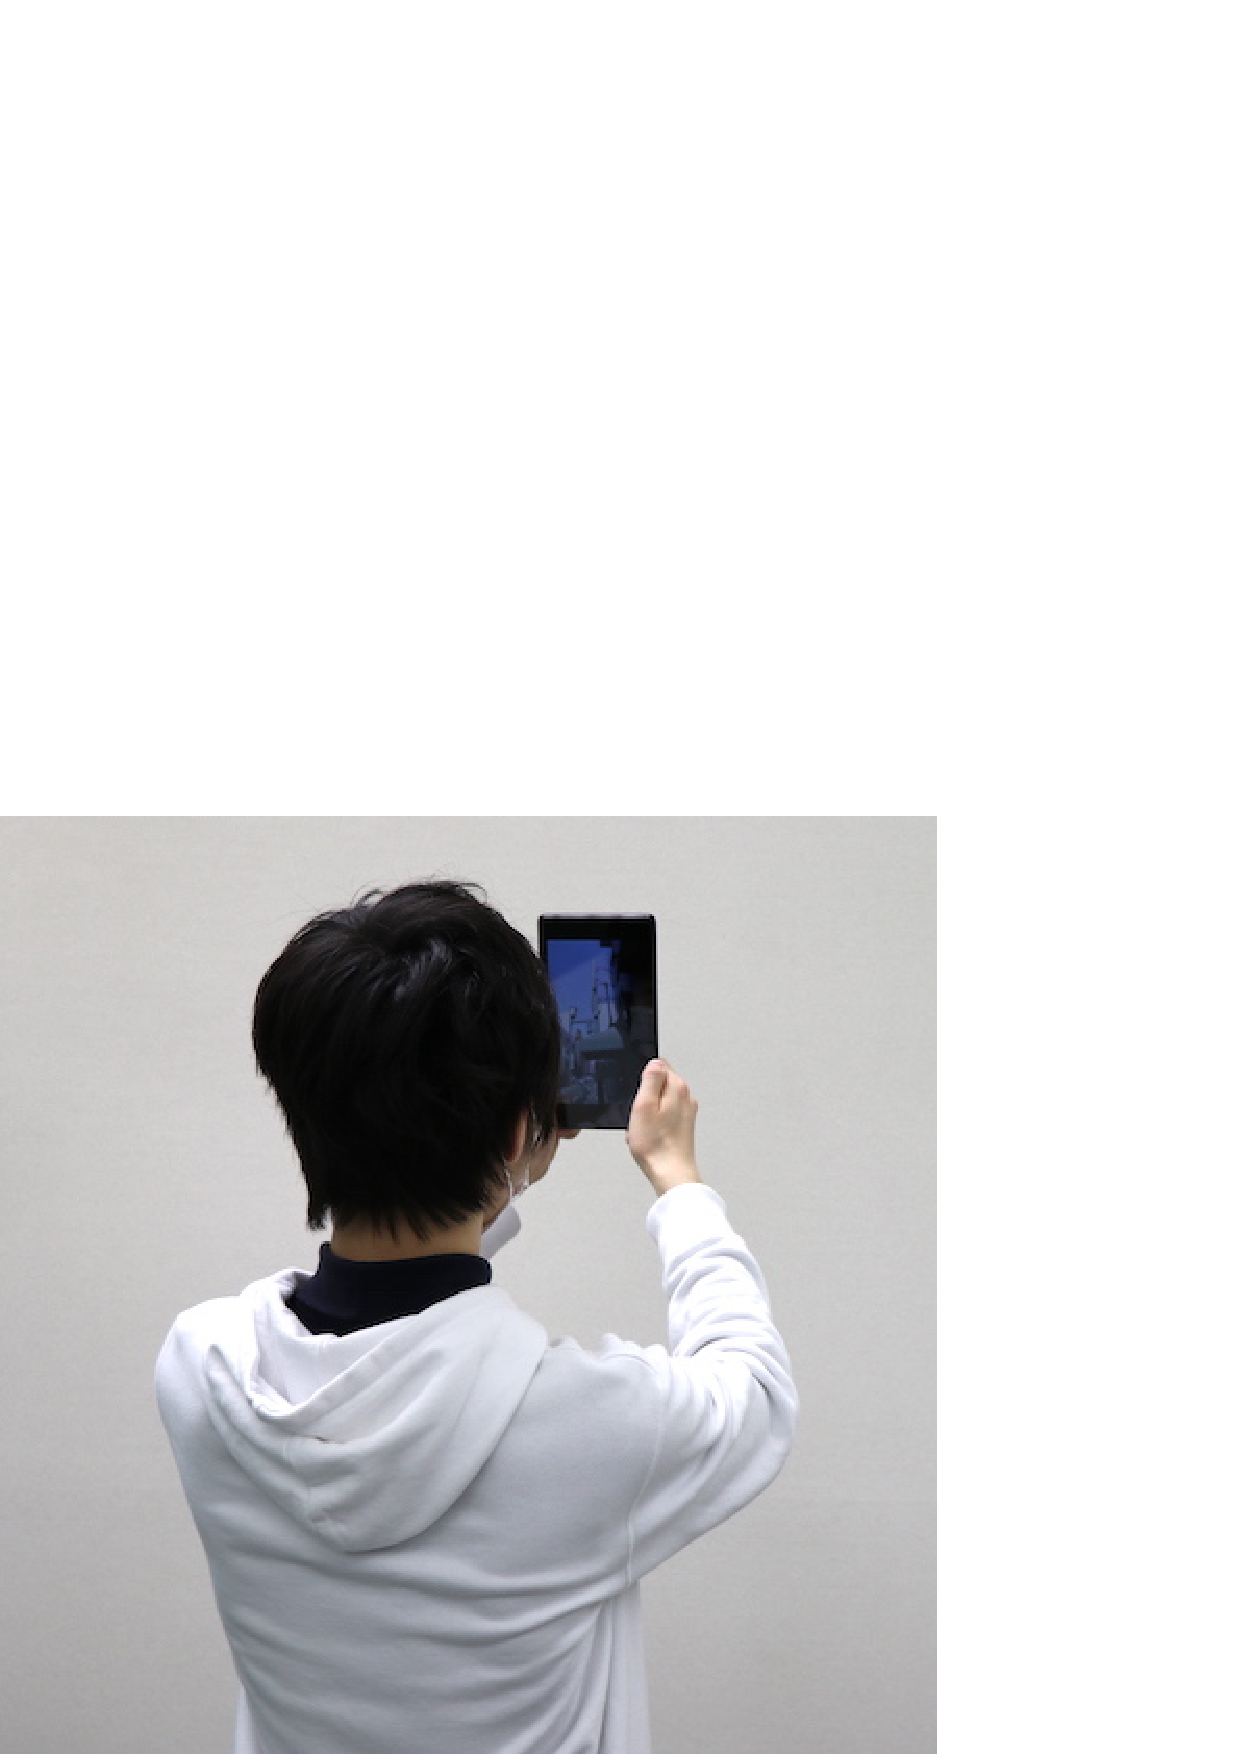
\includegraphics[width=\columnwidth, clip]{dr_exp.png}}
    \caption{実験風景(文献\cite{Kitamura:2017a}より図引用)}
    \label{figure:exp_dr_scenery}
  \end{figure}

  \begin{figure}[t]
    \begin{center}
      \begin{tabular}{cc}
        \begin{minipage}{0.45\hsize}
          \centering
          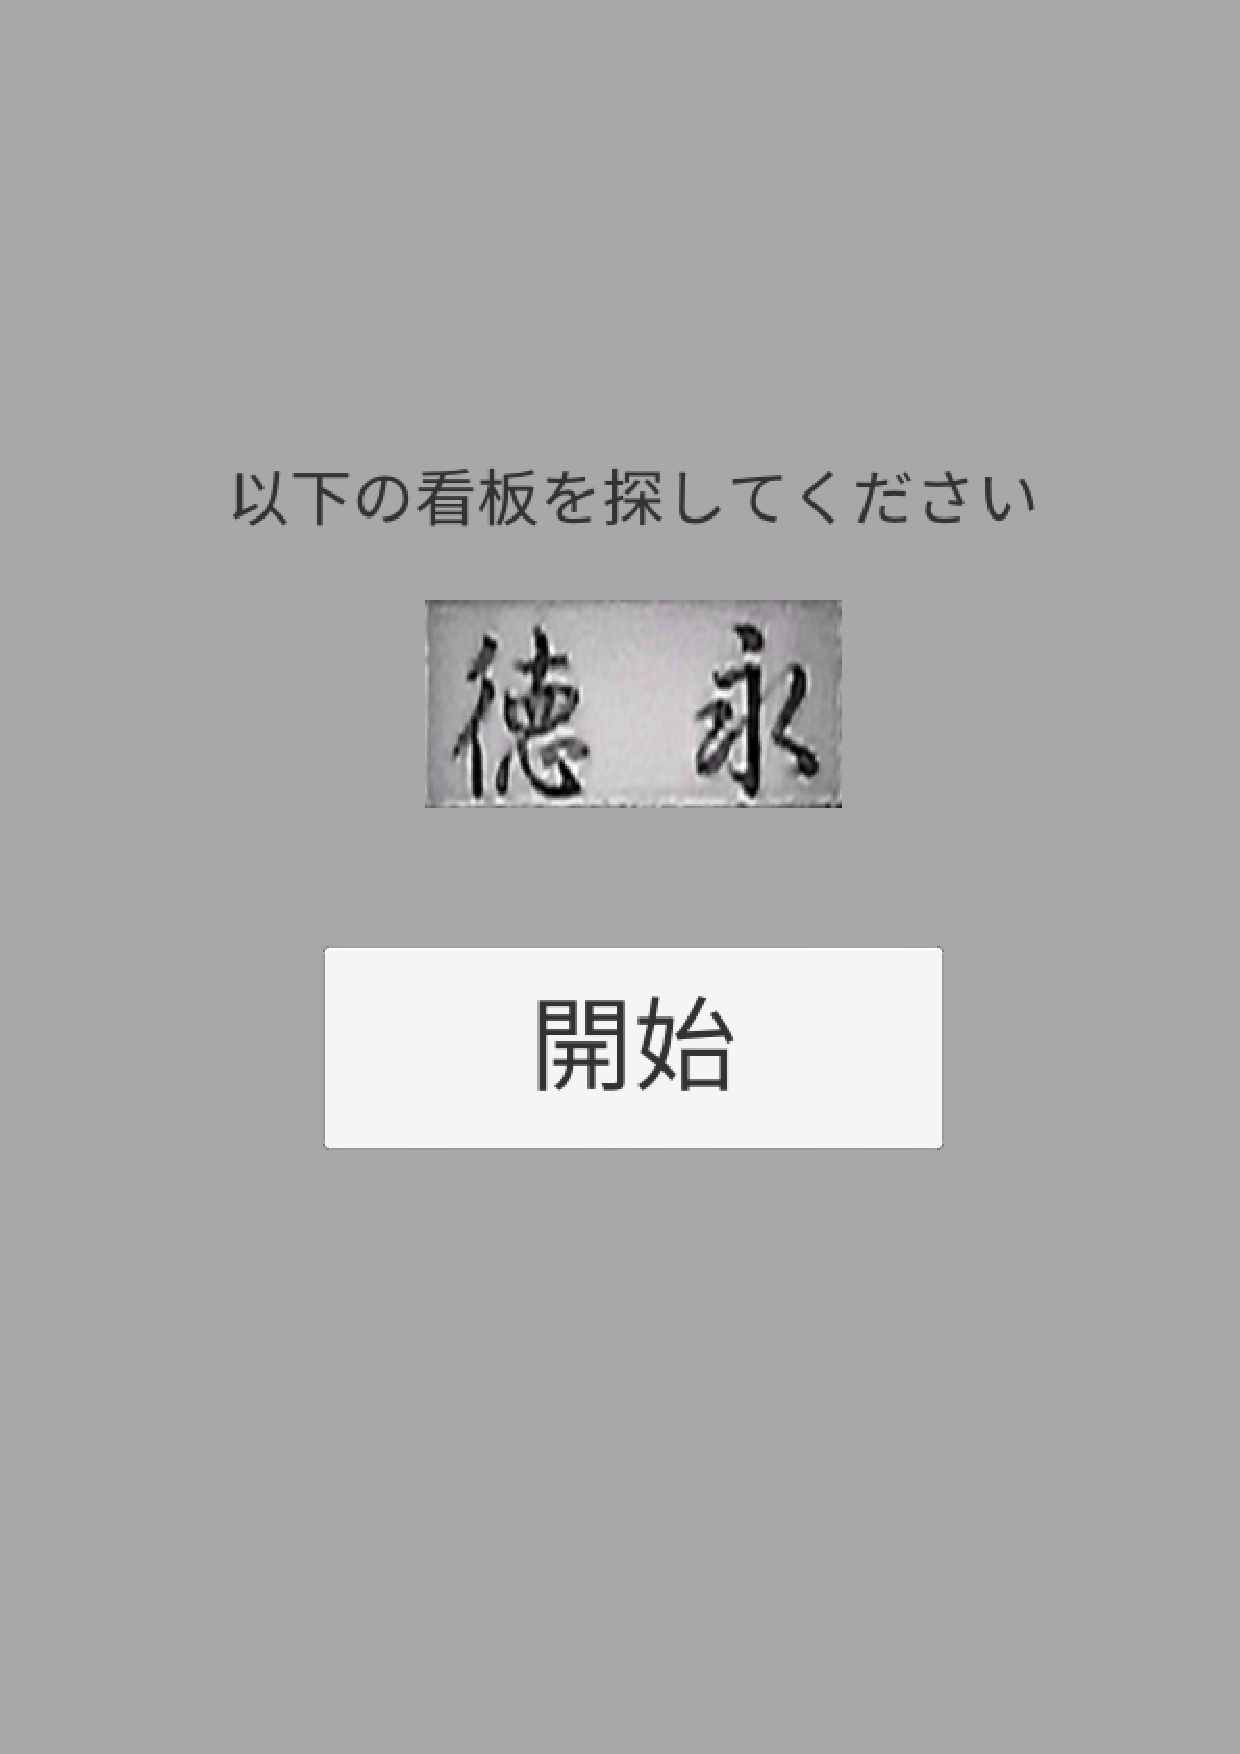
\includegraphics[clip, width=.9\textwidth]{dr_exp1.png}\\
          \small{(a)開始画面}
        \end{minipage}
        \begin{minipage}{0.45\hsize}
          \centering
          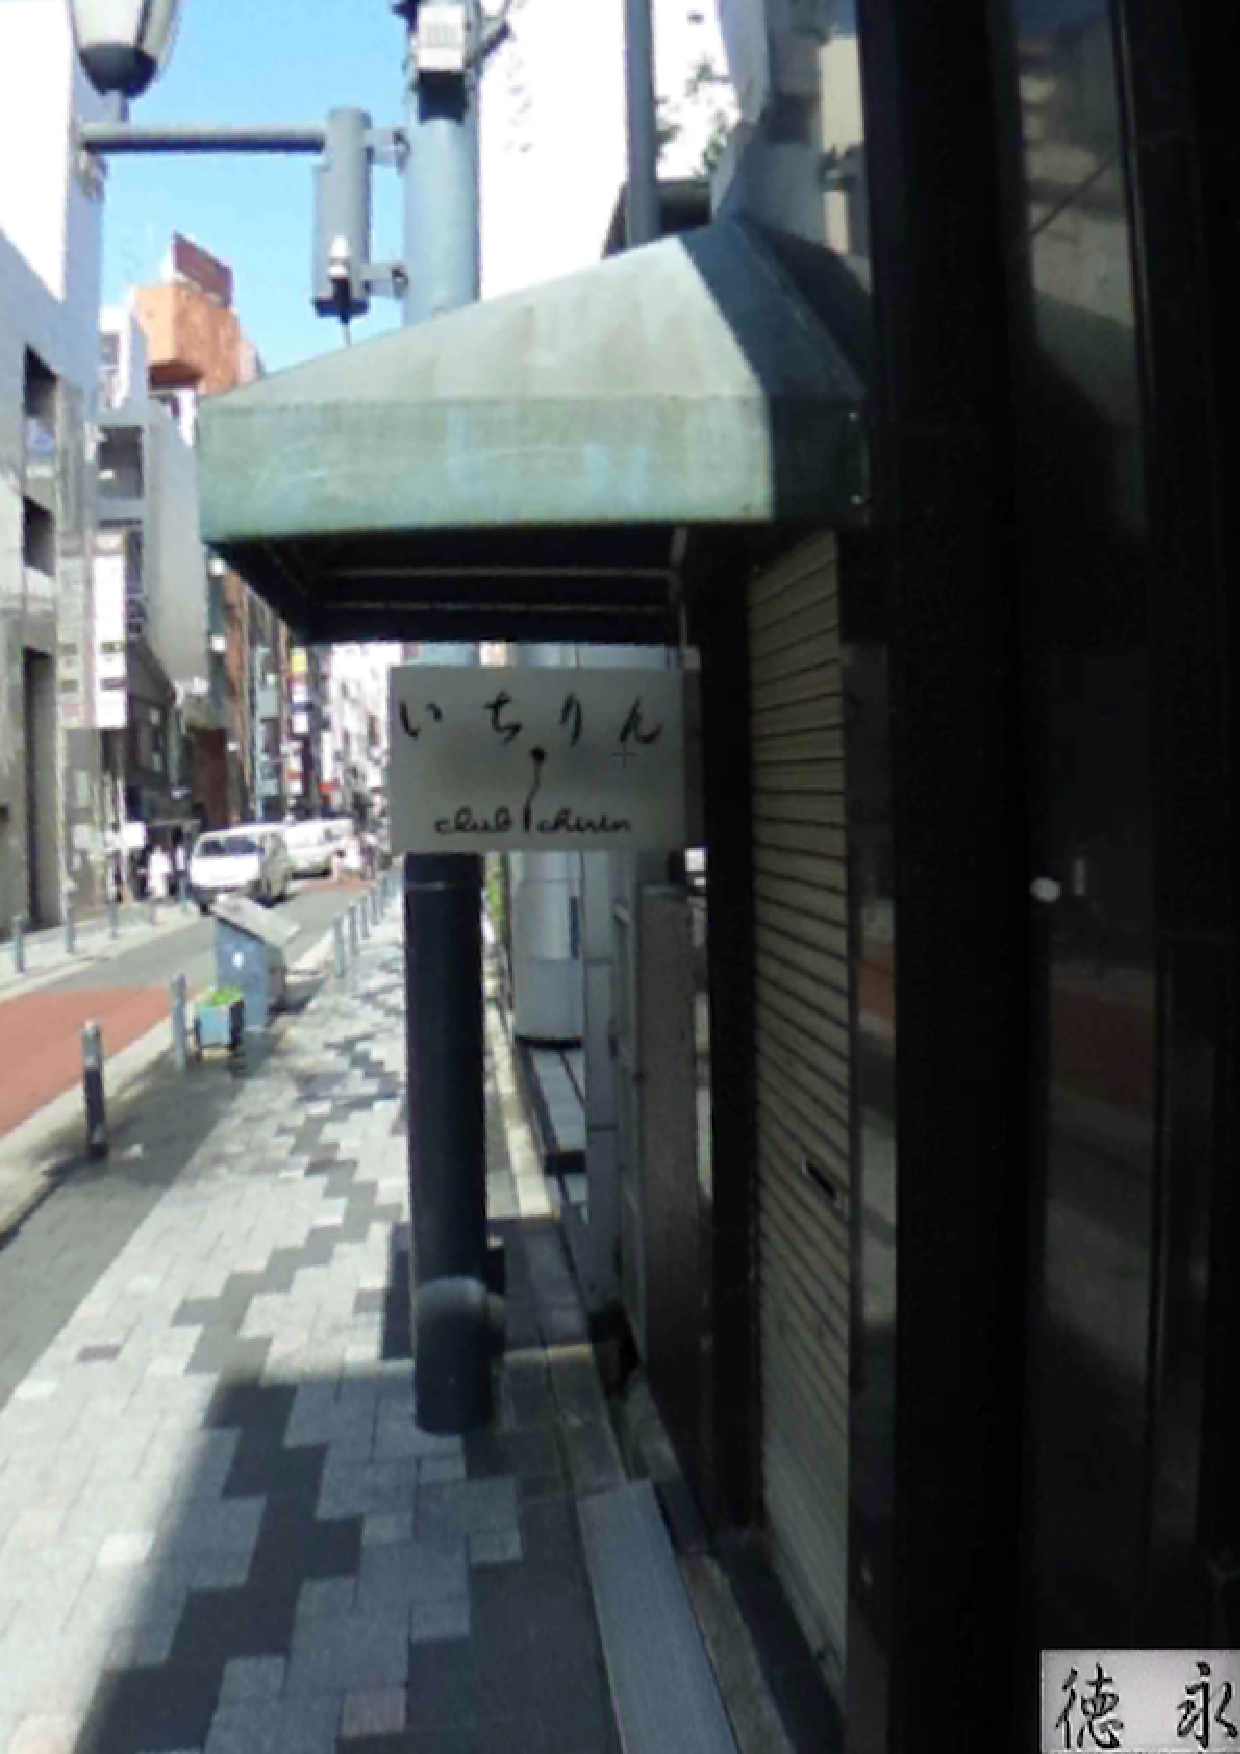
\includegraphics[clip, width=.9\textwidth]{dr_exp2.png}\\
          \small{(b)探索画面(1)}
        \end{minipage} \\\\
        \begin{minipage}{0.45\hsize}
          \centering
          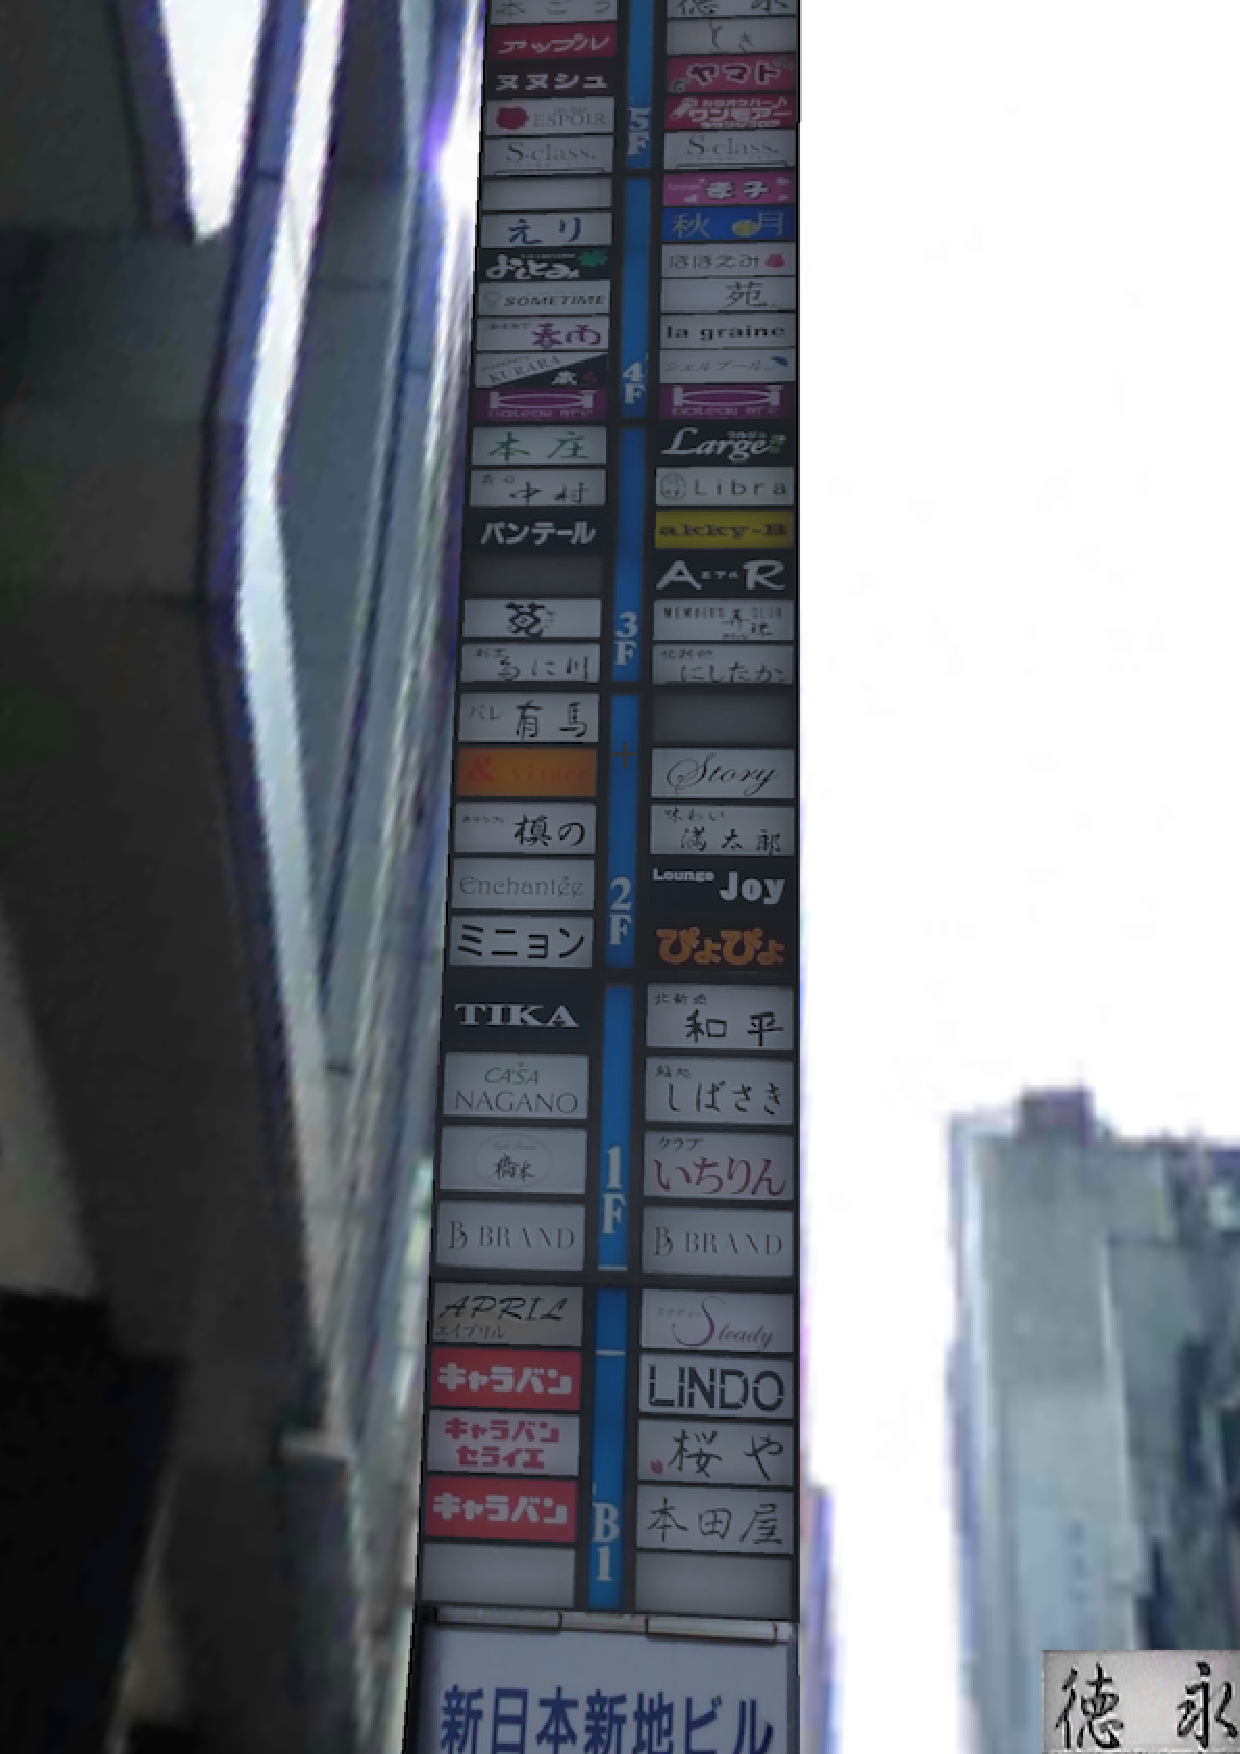
\includegraphics[clip, width=.9\textwidth]{dr_exp3.png}\\
          \small{(c)探索画面(2)}
        \end{minipage}
        \begin{minipage}{0.45\hsize}
          \centering
          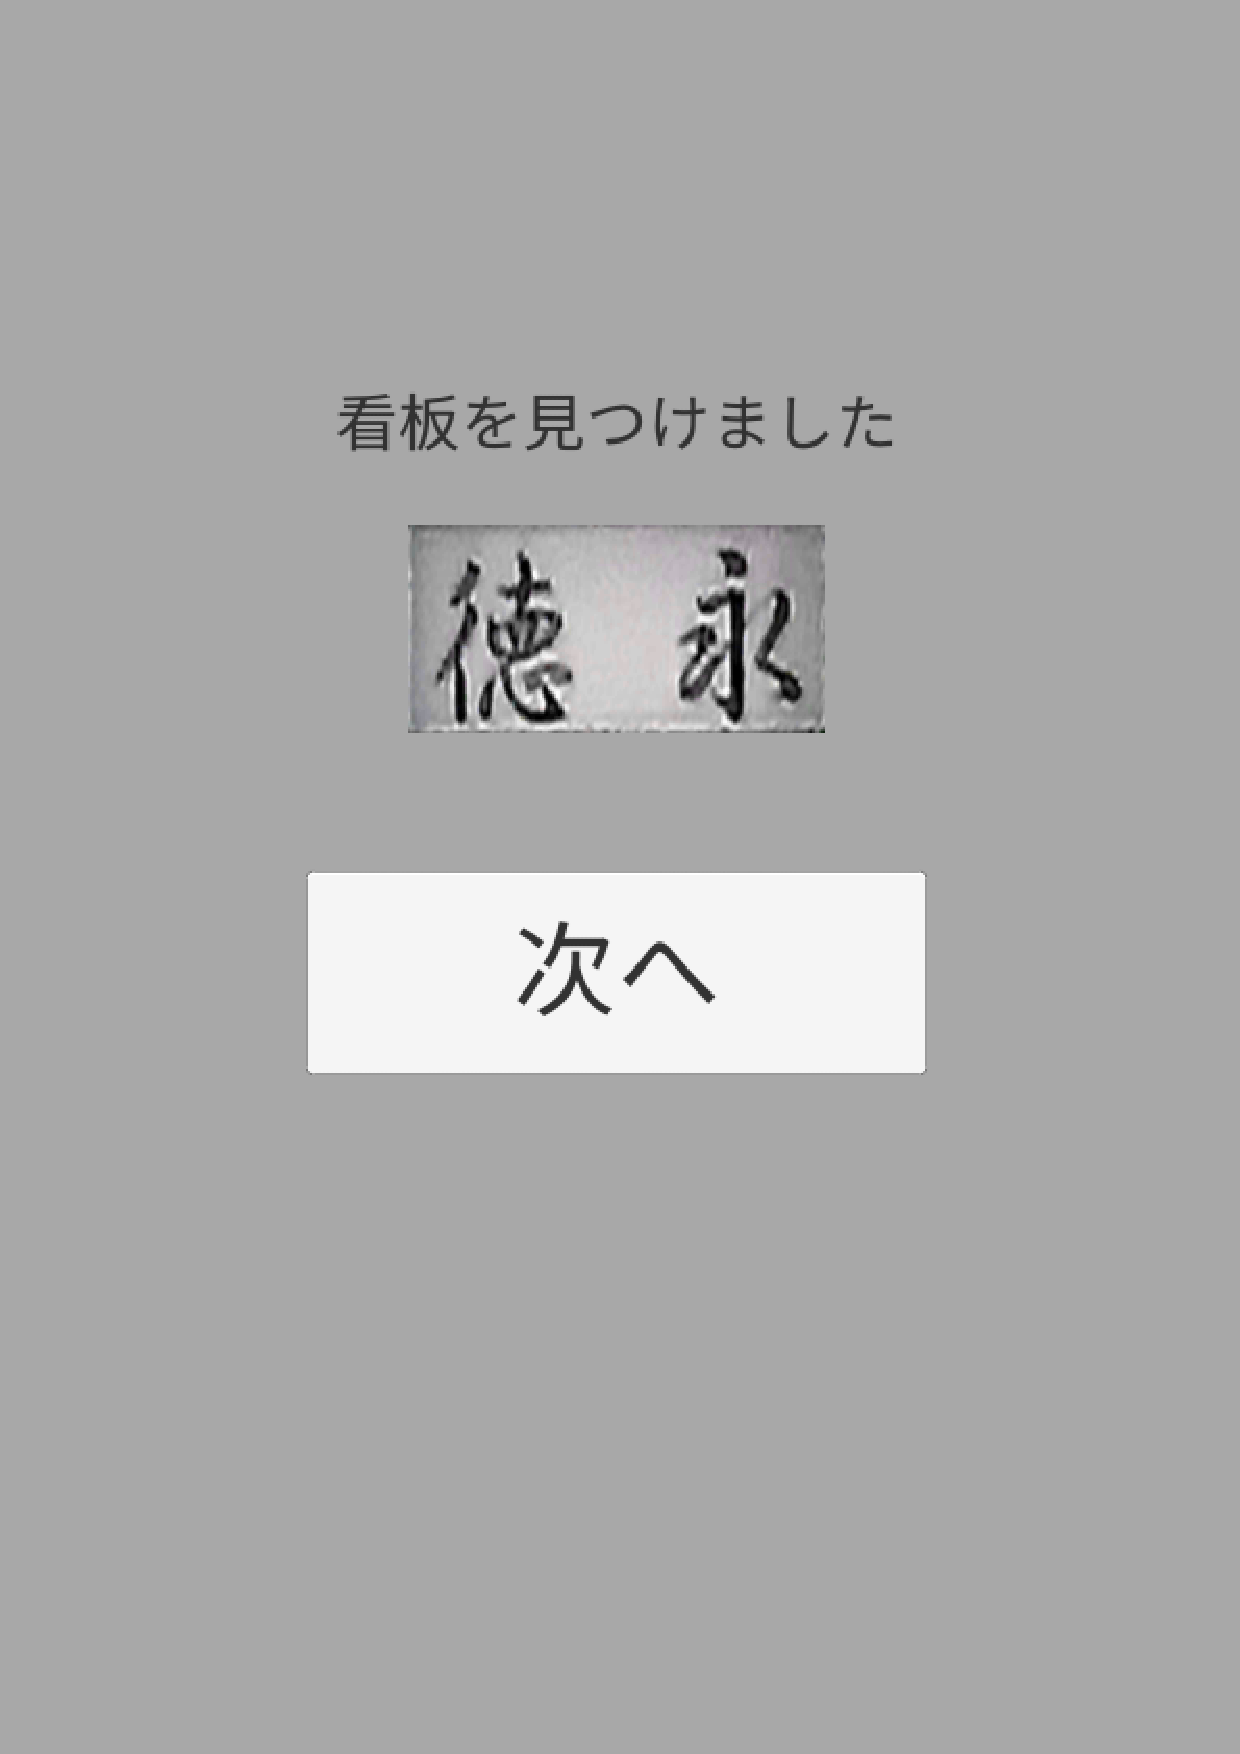
\includegraphics[clip, width=.9\textwidth]{dr_exp4.png}\\
          \small{(d)終了画面}
        \end{minipage}
      \end{tabular}
      \caption{実験の手順(文献\cite{Kitamura:2017a}より図引用)}
      \label{figure:exp_dr_procedure}
    \end{center}
  \end{figure}

\section{実験の結果}
  実験参加者が開始ボタンをタップしてから,指示された看板を全て見つけるまでの所要時間を計測し,通常型,加算型,減算型各々の探索時間とハイブリッド型の探索時間の平均値を比較した.その結果を以下に述べる.
  \subsection{時間帯が昼,探索対象が単体の場合}
    時間帯が昼,探索対象が単体の場合の探索時間を図\ref{figure:exp_dr_result_day} - (a) に示す.ハイブリッド型を用いた探索時間は,
    (1)通常型より有意に短い($t(22)=5.729, p<.05$)こと,
    (2)加算型より有意に短い($t(22)=2.852, p<.05$)ことが確認されたが,
    (3)減算型との間に有意差は見られなかった($t(22)=1.478, n.s.$).

  \subsection{時間帯が昼,探索対象が複数の場合}
    時間帯が昼,探索対象が複数の場合の探索時間を図\ref{figure:exp_dr_result_day} - (b) に示す.ハイブリッド型を用いた探索時間は,
    (1)通常型より有意に短い($t(22)=5.702, p<.05$)こと,
    (2)加算型より有意に短い($t(22)=6.144, p<.05$)こと,
    (3)減算型より有意に短い($t(22)=3.318, p<.05$)ことがそれぞれ確認された.

  \subsection{時間帯が夜,探索対象が単体の場合}
    時間帯が夜,探索対象が単体の場合の探索時間を図\ref{figure:exp_dr_result_night} - (a) に示す.ハイブリッド型を用いた探索時間は,
    (1)通常型より有意に短い($t(22)=4.325, p<.05$)こと,
    (2)加算型より有意に短い($t(22)=2.103, p<.05$)こと,
    (3)減算型より有意に短い($t(22)=2.485, p<.05$)ことがそれぞれ確認された.

  \subsection{時間帯が夜,探索対象が複数の場合}
    時間帯が夜,探索対象が複数の場合の探索時間を図\ref{figure:exp_dr_result_night} - (b) に示す.ハイブリッド型を用いた探索時間は,
    (1)通常型より有意に短い($t(22)=5.512, p<.05$)こと,
    (2)加算型との間に有意差はない($t(22)=1.857, n.s.$)こと,
    (3)減算型より有意に短い($t(22)=3.129, p<.05$)ことがそれぞれ確認された.

  \subsection{アンケート結果}
    実験終了後に,最も対象の看板を見つけやすかった提示手法についてアンケートを実施したところ,実験参加者の過半数が提案手法であるハイブリッド型情報提示手法を選択した.

  \begin{figure}[t]
    \begin{center}
      \begin{tabular}{cc}
        \begin{minipage}{0.45\hsize}
          \centering
          \includegraphics[clip, width=.95\textwidth]{dr_result1.eps}\\
          \small{(a)対象:単体}
        \end{minipage}
        \begin{minipage}{0.45\hsize}
          \centering
          \includegraphics[clip, width=.95\textwidth]{dr_result2.eps}\\
          \small{(b)対象:複数}
        \end{minipage}
      \end{tabular}
      \vspace{2pt}
      \caption{実験結果:昼($*:p<.05$)(文献\cite{Kitamura:2017a}より図引用)}
      \label{figure:exp_dr_result_day}
      \vspace{2cm}
      \begin{tabular}{cc}
        \begin{minipage}{0.45\hsize}
          \centering
          \includegraphics[clip, width=.95\textwidth]{dr_result3.eps}\\
          \small{(a)対象:単体}
        \end{minipage}
        \begin{minipage}{0.45\hsize}
          \centering
          \includegraphics[clip, width=.95\textwidth]{dr_result4.eps}\\
          \small{(b)対象:複数}
        \end{minipage}
      \end{tabular}
      \vspace{2pt}
      \caption{実験結果:夜($*:p<.05$)(文献\cite{Kitamura:2017a}より図引用)}
      \label{figure:exp_dr_result_night}
    \end{center}
  \end{figure}
\chapter{看板認識に関する評価実験}

\section{実験の目的}

\section{実験の概要}

\section{実験の手続き}

\section{実験の結果}

\section{考察}
\chapter{Search by Snapを用いたユーザ実験}
\section{実験の目的}
  ?章で述べたように,慣れていない地域や周囲の文字が読めないに状況おいて,ユーザが目の前にある店舗の情報や条件に合致する店舗の情報を瞬時に取得することは容易ではない.
  位置情報を手がかりに周囲の検索を行い,条件に合った店舗が見つかったとしても,ユーザ自身が居る環境と検索行為とが分断されているため,そのその環境からその店舗を探す手間が残るという問題点がある.
  そのため,提案システムを用いることによって,位置情報を利用したサービスと比較して店舗を簡単かつ直感的に探索できることを確認する.
  本稿では,地域に慣れていないユーザを対象に評価を行う前段階として,提案システムのユーザビリティを評価するために,地元の大学生を対象にユーザ実験を実施する.

\section{実験の概要}
  実験は大阪府高槻市にある高槻本通りにおいて,昼間にユーザが飲食店を探している状況を想定して行った.
  実験参加者は情報系の学部に通う大学生10名である.

  実験参加者にはタスク(A)として,「小だるま JR高槻駅前店」,「肉丼専門店 高槻肉劇場」,「磯丸水産 高槻店」の3店舗について,使用できるクレジットカードの種類を``Visa'',``Mastercard'',``JCB'',``American Express'',``Diners Club''の5つのチェックボックスから全て選択すること,タスク(B)として,「おだいどこはなれ 高槻店」,「高槻ちゃぶちゃぶ」,「赤から 高槻店」の3店舗について,月曜日の営業開始時刻を数値で入力すること,の2点を課した.
  タスク(A)は図\ref{fig:exp_point}中\textcircled{\scriptsize 1}で示した位置に立った状態,タスク(B)は図\ref{fig:exp_point}中\textcircled{\scriptsize 2}で示した位置に立った状態で行った.
  実験に用いた携帯端末はクアンタ・コンピュータ社\footnote{http://www.quantatw.com}のVA-10J(Android 5.0.2)である.
  提案システムとの比較対象とする位置情報を用いたサービスは,ランキングやユーザの口コミ・写真をもとにレストランの検索が行えるサービスである食べログ\footnote{https://tabelog.com}を用いた.

\begin{figure}[tb]
  \begin{center}
    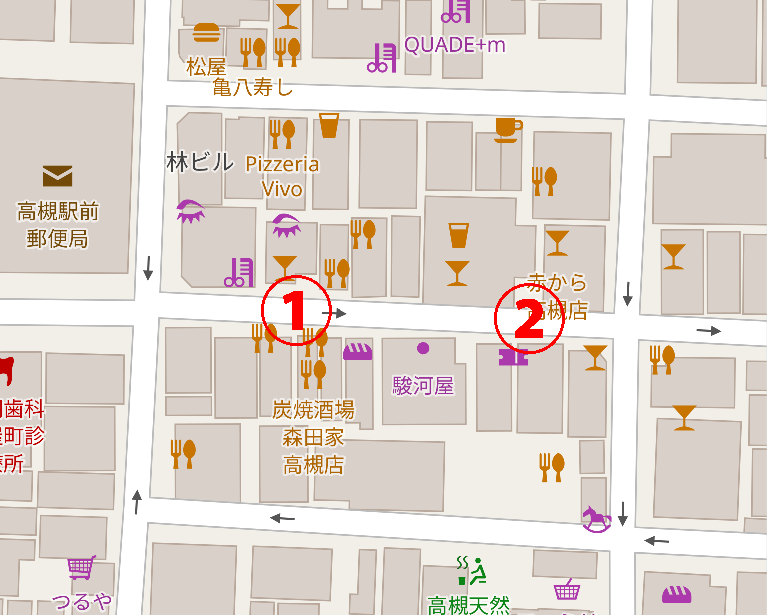
\includegraphics[clip, width=.95\columnwidth]{sbs_map_point.eps}
    \caption{実験の実施地点}
    \label{fig:exp_point}
  \end{center}
\end{figure}

\begin{figure}[t]
  \begin{minipage}{0.49\hsize}
    \begin{center}
      \includegraphics[clip, width=.95\textwidth]{sbs_interface.png}\\
      \caption{ユーザインタフェース}
      \label{fig:interface}
    \end{center}
  \end{minipage}
  \begin{minipage}{0.49\hsize}
    \begin{center}
      \includegraphics[clip, width=.95\textwidth]{sbs_exp_scenery.jpg}\\
      \caption{実験の風景}
      \label{fig:exp_scenery}
    \end{center}
  \end{minipage}
\end{figure}

\section{実験の手順}
  初めに,提案システムと食べログの使い方を実験参加者に説明する.
  次に,実験参加者に回答用フォームのURLを伝え,参加者は自身のスマートフォンでフォームを開く.
  実験に用いるシステムを起動した状態で参加者に実験用のスマートフォンを渡す.
  実験参加者はシステムを用いて求められている情報を探索し,フォームに入力して送信する.
  実験参加者がシステムの操作を始めてから送信ボタンをタップするまでの時間を計測する.
  実験の風景を図\ref{fig:exp_scenery}に示す.

  実験参加者をグループ(1)とグループ(2)に2分割し,グループ(1)にはタスク(A)を提案システム,タスク(B)を食べログを用いて行うよう指示を出し,グループ(2)にはタスク(A)を食べログ,タスク(B)を提案システムを用いて行うよう指示を出した.
  実験終了後には,参加者に「求めていた情報の見つけやすさ(簡便性)」,「情報探索の直感性(直感性)」について,食べログと提案システムとの間で5段階評価のアンケートへの回答を求めた.

\section{実験の結果}
  実験参加者がシステムに操作を初めてから指示された情報を全て収集し,送信ボタンをタップするまでの時間を計測し,タスク(A)とタスク(B)に関して提案システムを用いた場合と食べログを用いた場合とにおいて,探索時間の平均値を比較した.その結果を図\ref{fig:result_time}に示す.
  タスク(A)において,提案手法を用いた場合の探索時間は食べログを用いた場合よりも有意に短い($t(8)=2.343, p<.05$)ことが確認された.
  タスク(B)においても,提案手法を用いた場合の探索時間は食べログを用いた場合よりも有意に短い($t(8)=4.370, p<.05$)ことが確認された.

  各タスクにおいて,ユーザが正確に情報を収集できたかを測定するために,対象とした3店舗のうち,正確に情報を取得できた店舗数の割合を正解率として測定し,提案システムを用いた場合と食べログを用いた場合とにおいて,正解率の平均値を比較した.その結果を図\ref{fig:result_acc}に示す.
  タスク(A)において,提案手法を用いた場合と食べログを用いた場合とで,正解率に有意差は見られなかった($t(8)=1.000, n.s.$).
  タスク(B)においても,提案手法を用いた場合と食べログを用いた場合とで,正解率に有意差は見られなかった($t(8)=1.633, n.s.$).

  情報探索の簡便性と直感性について5段階のリッカート尺度を用い,「1」を「食べログ」,「5」を「提案システム」として5段階で回答してもらった.
  そのアンケート結果の分布を図\ref{fig:result_question}に示す.
  簡便性に関する平均値は4.4,直感性に関する平均値は4.5であった.

  \begin{figure}[tb]
    \begin{center}
      \includegraphics[clip, width=.95\columnwidth]{sbs_result_time.pdf}
      \caption{探索時間}
      \label{fig:result_time}
    \end{center}
  \end{figure}
  \begin{figure}[tb]
    \begin{center}
      \includegraphics[clip, width=.95\columnwidth]{sbs_result_acc.pdf}
      \caption{正解率}
      \label{fig:result_acc}
    \end{center}
  \end{figure}
  \begin{figure}[tb]
    \begin{center}
      \includegraphics[clip, width=.95\columnwidth]{sbs_result_question.pdf}
      \caption{アンケート(1: 食べログ〜 5: 提案システム)}
      \label{fig:result_question}
    \end{center}
  \end{figure}

\section{議論}
\label{sec:discussion}
\subsection{実験結果に関して}
  実験結果から,情報探索時間に関しては,本稿で扱ったいずれの場合においても,提案システムを用いた場合は食べログを用いた場合よりも探索時間が有意に短くなることが明らかとなった.このことから,提案システムを用いることによって,位置情報のみを用いた場合と比較してユーザはより素早く求めている情報を取得することが可能になるといえる.
  情報探索の正確さに関しては,本稿で扱ったいずれの場合においても,提案システムを用いた場合と食べログを用いた場合とでは正解率に有意差は見られなかった.このことから,言語障壁がなければ位置情報のみを用いても正確に情報を探索することが可能であり,提案システムを用いた場合においても正確な情報探索が可能であるといえる.
  また,アンケート結果から,提案システムを用いることによって,位置情報のみを用いた場合と比較してより簡単かつ直感的に情報が探索できるようになることが示唆された.

\subsection{提案システムで達成されたこと}
  提案システムを用いることによって,本研究の目的である,ユーザの目の前にある店舗の情報を直感的かつ簡単に取得できることが達成されたと考えられる.
  これにより,?章で述べた,慣れていない地域においても,ユーザが求める条件に合致する店舗を探索できるようになることが示唆された.

\subsection{課題}
\label{sec:limitation}
  本研究の課題として,(1)OSMのノードと看板画像を手作業で関連付けなければならない点,(2)インターネット上の情報から多種多様な店舗の看板画像を大量に集めることは困難であるため,手作業で看板画像を1店舗につき100枚程度集めなければならない点,が挙げられる.
  (1)に対しては,看板画像を提示してユーザに店舗名を回答するシステムを実装することで解決でき,(2)に対してはユーザに店舗の看板画像を提示し,それと同じ写真を撮影して投稿するシステムを実装することで解決できると考えられる.
  これらのシステムにゲーミフィケーションを利用し,ユーザの行動に対して報酬を与えることによって,多数のデータを効率よく収集できると考えられる.

\subsection{今後の展望}
  今後の展望として,看板認識をサーバ上で行うのではなく,Tiny--YOLO等を用いて携帯端末上で行うことを検討する.これにより,サーバへ画像を送信する必要がなくなるため,通信量の大幅な軽減が期待される.
  また,OSMのデータは誰もが編集可能であるため,\ref{sec:limitation}節で述べたように,その地域に慣れている地元のユーザが自身でデータを収集し,OSMを通して活用できるようになる枠組みの構築を目指す.
  OSMのノードには``cuisine''タグが存在し,``burger'',``noodle'',``japanese'',``chinese''など,飲食店で提供される食品の種類を表す値を追加できる.他にもベジタリアン向けのメニューが提供されていることを表す``diet:vegetarian''や,イスラム教の戒律で許されている食品のみを使用したメニューが提供されていることを表す``diet:halal''などのタグも存在する.
  さらに,店舗名の英語またはローマ字表記を表す``name:en''タグや中国語表記の``name:zh''タグ,韓国語表記の``name:ko''タグなどを充実させることによって,ユーザインタフェースを多言語に対応させることが可能となる.
  これらのデータを活用することにより,その地域に慣れていない人や,地元の文字が読めない外国人観光客に対して,求めている情報を容易に取得でき,アレルギーや宗教的制約などの理由による食事制限にも対応可能なナビゲーションを実現できる.
  
  本稿における実験参加者は地元の大学生であるため,地域に慣れていないユーザや非漢字圏など地元の文字が読めないユーザを対象としたユーザ実験を実施する.

\chapter{議論}
\label{chapter:discussion}

\chapter{結論}
\label{chapter:conclusion}
  本研究の目的は,〜である.
  以下の本稿の内容を纏める.

  \ref{chapter:introduction}章では,

  \ref{chapter:relatedwork}章では,

  \ref{chapter:design_guidline}章では,

  \ref{chapter:implement_dr}章では,

  \ref{chapter:implement_recog}章では,

  \ref{chapter:implement_sbs}章では,

  \ref{chapter:experiment_dr}章では,

  \ref{chapter:experiment_sbs}章では,

  \ref{chapter:discussion}章では,

%
% thanks.tex
%
\chapter*{謝辞}



\bibliographystyle{ipsjsort}
\bibliography{reference}


\end{document}